\subsection{Interpolazione trigonometrica}

Nel caso di funzioni periodiche, ad esempio con periodo $2\pi$ e con $f\left(0\right) = f\left(2\pi\right)$, si ha il valore delle ascisse pari a:
\begin{equation*}
	x_{j} = \dfrac{2\pi j}{\left(n+1\right)} \hspace{2em} j = 0, \dots, n
\end{equation*}
In questo caso, l'interpolatore Lagrangiano non approssima in modo ottimale la funzione $f$ lontana dai nodi, dato che è un polinomio di grado $n$ (per cui in generale non periodico!).

\highspace
Supponendo $n$ pari e $M = \frac{n}{2}$, si può costruire l'\definition{interpolatore trigonometrico $\tilde{f}\left(x\right)$} come la \textbf{combinazione lineare di seni e coseni}:
\begin{equation}\label{eq: interpolatore trigonometrico}
	f\left(x\right) = \dfrac{a_{0}}{2} + \displaystyle\sum_{k=1}^{M} \left[a_{k} \cos\left(kx\right) + b_{k} \sin\left(kx\right)\right]
\end{equation}
Per opportuni coefficienti complessi incogniti $a_{k}$, per $k = 0, \dots, M$ e $b_{k}$ per $k = 1, \dots, M$. Come si può vedere, la funzione periodica $\tilde{f}\left(x\right)$ è di periodo $2\pi$ caratterizzata da $M+1$ \textbf{frequenze} e \textbf{coefficienti} $a_{k}$ e $b_{k}$ con $k = 0, \dots, M$.

\highspace
\textbf{Sfruttando} la nota formula di \textbf{Eulero}:
\begin{equation*}
	e^{ikx} = \cos\left(kx\right) + i\sin\left(kx\right)
\end{equation*}
L'\textbf{interpolatore trigonometrico} può essere riscritto in modo più compatto:
\begin{equation}\label{eq: interpolatore trigonometrico con Eulero}
	\tilde{f}\left(x\right) = \displaystyle\sum_{k = -M}^{M} c_{k} e^{ikx}
\end{equation}
Inoltre, dall'equazione \ref{eq: interpolatore trigonometrico} i valori $a_{k}, b_{k}$ con $k = 0, \dots, M$ sono:
\begin{equation*}
	\begin{cases}
		a_{k} = c_{k} + c_{-k} \\
		b_{k} = i\left(c_{k} - c_{-k}\right)
	\end{cases}
\end{equation*}
E nell'interpolazione trigonometrica con Eulero \ref{eq: interpolatore trigonometrico con Eulero} si ha:
\begin{equation*}
	\begin{cases}
		c_{k} = \frac{1}{2}\left(a_{k} - ib_{k}\right) \\
		c_{-k} = \frac{1}{2}\left(a_{k} + ib_{k}\right)
	\end{cases}
\end{equation*}
Quindi, le funzioni interpolatrici trigonometriche $\tilde{f}\left(x\right)$ sono $2M+1 = n+1$ equazioni nelle $n+1$ incognite $c_{k}$.

\highspace
La \textbf{distanza} (costante) fra due nodi $h = \frac{2\pi}{\left(n+1\right)}$ come:
\begin{equation*}
	x_{j} = jh \hspace{2em} j = 0, \dots, n
\end{equation*}
Si impone inoltre il \textbf{vincolo di interpolazione}:
\begin{equation}\label{eq: vincolo di interpolazione}
	\tilde{f}\left(x_{j}\right) = \displaystyle\sum_{k = -M}^{M} c_{k}e^{ikjh} = f\left(x_{j}\right) \hspace{2em} j = 0, \dots, n
\end{equation}
A differenza dell'interpolazione Lagrangiana, i coefficienti della combinazione lineare $c_{k}$ con $k = -M, \dots, M$, sono incogniti. Si hanno di conseguenza $n+1$ equazioni nelle $2M + 1 = n+1$ incognite $c_{k}$. Tale equazione è una base di partenza per le formule nei paragrafi successivi.

\newpage

\subsubsection{Trasformata Discreta di Fourier}

Dato un intero $m \in \left[-M, M\right]$, si moltiplica all'equazione di base \ref{eq: vincolo di interpolazione}, a pagina \pageref{eq: vincolo di interpolazione}, a sinistra e a destra per $e^{-imx_{j}} \Rightarrow e^{imjh}$ e si sommano su $j$:
\begin{equation}
	\displaystyle\sum_{j=0}^{n}\sum_{k=-M}^{M} c_{k} e^{ikjh} e^{-imjh} = \sum_{j=0}^{n} f\left(x_{j}\right) e^{-imjh}
\end{equation}
In cui si può esporre una relazione esplicita fra i coefficienti e i valori noti della funzione $f\left(x_{j}\right)$:
\begin{equation}
	c_{m} = \dfrac{1}{n+1} \displaystyle\sum_{j=0}^{n} f\left(x_{j}\right) e^{-imjh} \hspace{2em} m = -M, \dots, M
\end{equation}
La funzione $f\left(x_{j}\right)$ viene chiamata \definition{Trasformata discreta di Fourier (DFT)}. \textbf{Queste sono $n+1$ equazioni nelle incognite $f\left(x_{j}\right)$}.

\highspace
Parlando di DTF, è necessario introdurre anche lo \textbf{spazio fisico} e delle \textbf{frequenze}. Dati i vettori $\mathbf{c} \in \mathbb{R}^{n+1}$ di componenti $c_{k}$ e $\mathbf{f} \in \mathbb{R}^{n+1}$ di componenti $f\left(x_{j}\right)$, è possibile riscrivere la trasformata di Fourier nello \textbf{spazio delle frequenze} $k$ come:
\begin{equation*}
	c_{k} = \dfrac{1}{n+1} \displaystyle\sum_{j=0}^{n} f\left(x_{j}\right) e^{-ikjh} \hspace{2em} k = -M, \dots, M
\end{equation*}
E in forma matriciale nel seguente modo:
\begin{equation}
	\mathbf{c} = T\mathbf{f}
\end{equation}
Con la matrice $T$ composta da elementi:
\begin{equation*}
	T_{kj} = \dfrac{1}{n+1} e^{-ikjh}
\end{equation*}

\highspace
Nel caso in cui si vuole passare dallo \textbf{spazio delle frequenze} $f\left(x_{j}\right)$ allo \textbf{spazio fisico} $c_{k}$, si può usare il vincolo di interpolazione (eq. \ref{eq: vincolo di interpolazione}, pag. \pageref{eq: vincolo di interpolazione}):
\begin{equation*}
	\tilde{f}\left(x_{j}\right) = \displaystyle\sum_{k = -M}^{M} c_{k}e^{ikjh} \hspace{2em} j = 0, \dots, n
\end{equation*}
E in forma matriciale nel seguente modo:
\begin{equation}
	\mathbf{f} = T^{-1} \mathbf{c}
\end{equation}
Con la matrice $T^{-1}$ composta da elementi:
\begin{equation*}
	\left(T^{-1}\right)_{kj} = e^{ikjh}
\end{equation*}
La \textbf{trasformazione dallo spazio delle frequenze allo spazio fisico} è chiamata \definition{Trasformata Discreta di Fourier inversa (Inverse Discrete Fourier Transform, IDFT)}.

\newpage

\subsubsection{Fast Fourier Transform (FFT)}

Il calcolo dei coefficienti $c_{k}$ può essere fatto ancora più rapidamente utilizzato la \definition{Trasformata rapida di Fourier (Fast Fourier Transform, FFT)}.

\highspace
Si consideri una generica matrice quadrata $A$ di dimensione $\left(n+1\right) \times \left(n+1\right)$ e un vettore $\mathbf{x}$ di dimensione $n+1$. È possibile calcolare la componente $w_{j}$ del vettore $\mathbf{w} = A\mathbf{x}$ come:
\begin{equation}
	w_{j} = \displaystyle\sum_{k=1}^{n} A_{jk} x_{k}
\end{equation}

\highspace
Nella FFT, la matrice $T$ ha una struttura particolare chiamata di Toeplitz. Questo comporta che l'elemento $w_{j}$ del vettore $\mathbf{w} = T\mathbf{x}$ è determinato solo dagli elementi della matrice $T$, ovverosia $T_{km}$ (con $j = km$). Una struttura tipica della matrice è:
\begin{equation*}
	T = \dfrac{1}{n+1} \begin{bmatrix}
		e^{-ih} & e^{-2ih} & e^{-3ih} & \cdots & \cdots & e^{-nih} \\
		e^{-2ih} & e^{-4ih} & e^{-6ih} & \cdots & \cdots & e^{-2nih} \\
		e^{-3ih} & e^{-6ih} & e^{-9ih} & \cdots & \cdots & e^{-3nih} \\
		\vdots & & \ddots & & & \vdots \\
		\vdots & & \ddots & & & \vdots \\
		e^{-nih} & e^{-2nih} & e^{-3nih} & \cdots & \cdots & e^{-n^{2}ih}
	\end{bmatrix}
\end{equation*}
Il \textbf{costo computazione} del vettore $\mathbf{w}$, a causa della forma particolare della matrice di Toeplitz, è uguale a \underline{$n \log_{2} n$ operazioni}.

\longline

\subsubsection{Espressione Lagrangiana dell'interpolatore trigonometrico}\index{interpolatore trigonomentrico in forma Lagrangiana}

L'interpolatore trigonometrico può essere scritto in forma Lagrangiana, ovvero con coefficienti nella combinazione lineare dati dal risultato dei vari $f\left(x_{j}\right)$, nel seguente modo:
\begin{equation}
	\tilde{f}\left(x\right) = \displaystyle\sum_{j=0}^{n} f\left(x_{j}\right) \varphi_{j}^{T}\left(x\right)
\end{equation}
Dove il polinomio $\varphi$ non è altro che:
\begin{equation}
	\varphi_{j}^{T}\left(x_{k}\right) = \delta_{jk}
\end{equation}

\begin{flushleft}
	\textcolor{Green3}{\faIcon{question-circle} \textbf{E in questo caso la convergenza?}}
\end{flushleft}
La convergenza è possibile esprimerla tramite il seguente teorema.
\begin{theorem}
	Si supponga che la funzione $f\left(x\right)$ ammetta derivata continua e periodica di periodo $2\pi$ fino all'ordine $s+1$ compreso.
	
	Allora, si ha il seguente risultato di \definition{convergenza per l'interpolatore trigonometrico in forma Lagrangiana}:
	\begin{equation}
		\underset{x \in \left[0, 2\pi\right]}{\max} \left|f\left(x\right) - \tilde{f}\left(x\right)\right| \le C\dfrac{1}{n^{s}}
	\end{equation}
	Per un'opportuna costante $C$.
\end{theorem}

\noindent
Dal precedente teorema, se ne deriva che la \textbf{convergenza è esponenziale qualora il precedente risultato valga per} $\forall s > 0$.

\newpage

\subsubsection{Fenomeno dell'aliasing e teorema di Shannon}

Se il numero di dati $n+1$ non è sufficientemente elevato, l'\textbf{interpolatore trigonometrico non è in grado di descrivere le frequenze $k$ più alte}. Questo problema viene chiamato \definition{fenomeno di aliasing}.

\highspace
Nel mondo reale, l'occhio umano campiona con una frequenza massima le informazioni luminose che provengono dal mondo esterno. Ma se tale campionamento non è sufficientemente frequente da catturare la frequenza massima del fenomeno esterno, allora l'immagine riprodotta dal cervello (che di fatto agisce in questo caso come un interpolatore trigonometrico) sarà caratterizzata da frequenze diverse (aliasing). E questo è anche il motivo per negli elicotteri si vedono le pale girare molto lentamente o addirittura in senso opposto.

\highspace
In particolare, sia $k_{\max}$ la \textbf{frequenza massima} della funzione $f\left(x\right)$. Se $n \le 2k_{\max}$, la \textbf{frequenza massima dell'interpolatore trigonometrico} $\tilde{f}\left(x\right)$ è minore di $k_{\max}$ (aliasing).

\begin{examplebox}[: aliasing]
	Gli effetti dell'aliasing si possono vedere confrontando, per esempio, le seguenti due funzioni:
	\begin{itemize}
		\item In linea continua:
		\begin{equation*}
			f\left(x\right) = \sin\left(x\right) + \sin\left(5x\right)
		\end{equation*}
		
		\item Linea tratteggiata, l'interpolatore trigonometrico $\tilde{f}\left(x\right)$ con $M=3$
	\end{itemize}
	
	\begin{center}
		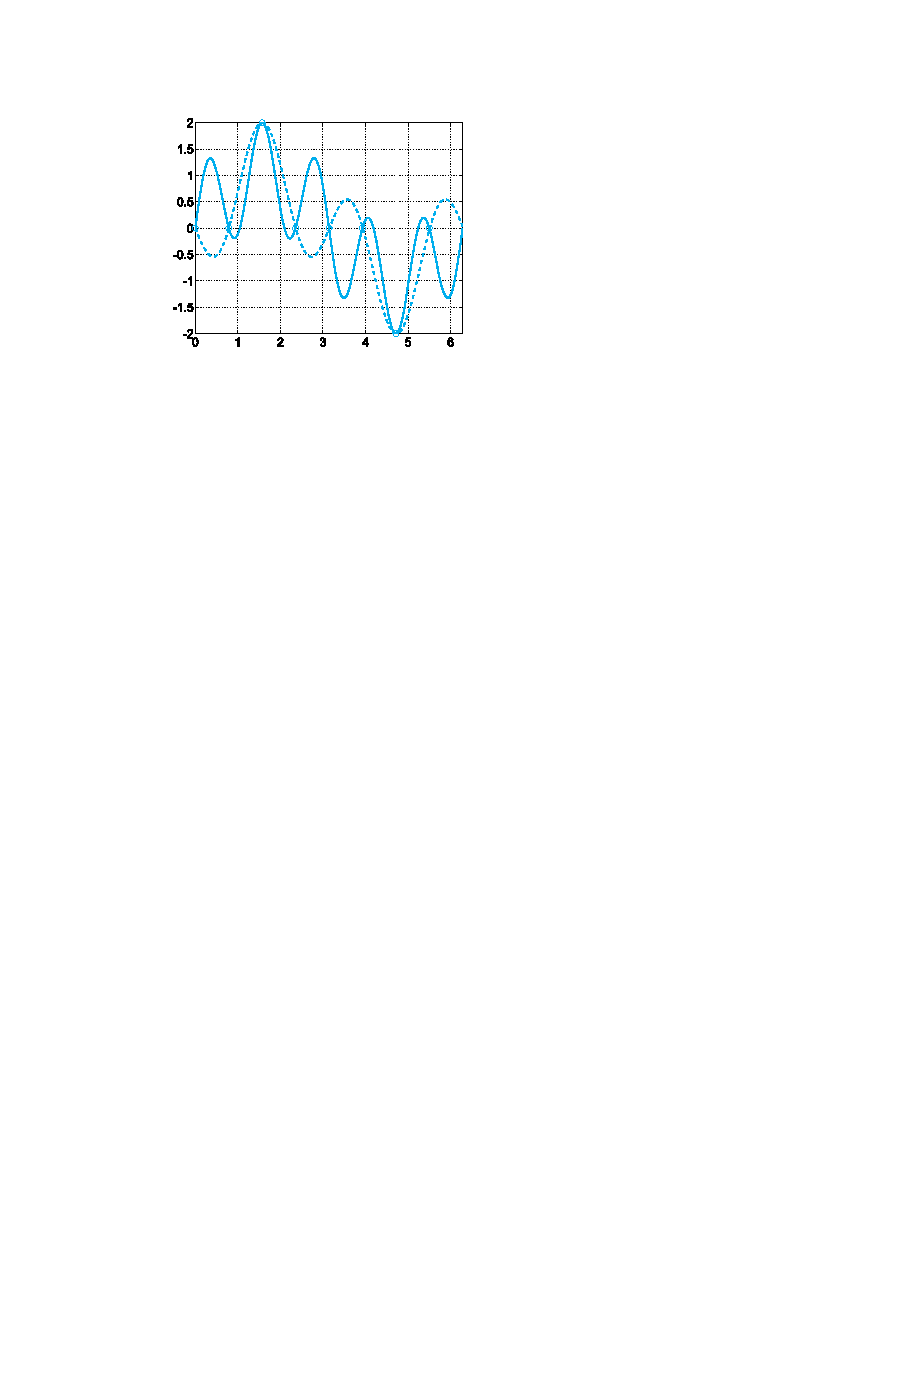
\includegraphics[width=.5\textwidth]{img/aliasing-1.pdf}
	\end{center}
\end{examplebox}

\noindent
Quindi, il \definition{teorema di Shannon} afferma che $n$ deve essere:
\begin{equation}
	n > 2k_{\max}
\end{equation}